\documentclass[11pt,a4paper]{report}
\usepackage[textwidth=37em,vmargin=30mm]{geometry}
\usepackage{calc,xunicode,amsmath,amssymb,paralist,enumitem,tabu,booktabs,datetime2,xeCJK,xeCJKfntef,listings}
\usepackage{tocloft,fancyhdr,tcolorbox,xcolor,graphicx,eso-pic,xltxtra,xelatexemoji}

\newcommand{\envyear}[0]{2025}
\newcommand{\envdatestr}[0]{2025-09-19}
\newcommand{\envfinaldir}[0]{webdb/2025/20250919/final}

\usepackage[hidelinks]{hyperref}
\hypersetup{
    colorlinks=false,
    pdfpagemode=FullScreen,
    pdftitle={Web Digest - \envdatestr}
}

\setlength{\cftbeforechapskip}{10pt}
\renewcommand{\cftchapfont}{\rmfamily\bfseries\large\raggedright}
\setlength{\cftbeforesecskip}{2pt}
\renewcommand{\cftsecfont}{\sffamily\small\raggedright}

\setdefaultleftmargin{2em}{2em}{1em}{1em}{1em}{1em}

\usepackage{xeCJK,xeCJKfntef}
\xeCJKsetup{PunctStyle=plain,RubberPunctSkip=false,CJKglue=\strut\hskip 0pt plus 0.1em minus 0.05em,CJKecglue=\strut\hskip 0.22em plus 0.2em}
\XeTeXlinebreaklocale "zh"
\XeTeXlinebreakskip = 0pt


\setmainfont{Brygada 1918}
\setromanfont{Brygada 1918}
\setsansfont{IBM Plex Sans}
\setmonofont{JetBrains Mono NL}
\setCJKmainfont{Noto Serif CJK SC}
\setCJKromanfont{Noto Serif CJK SC}
\setCJKsansfont{Noto Sans CJK SC}
\setCJKmonofont{Noto Sans CJK SC}

\setlength{\parindent}{0pt}
\setlength{\parskip}{8pt}
\linespread{1.15}

\lstset{
	basicstyle=\ttfamily\footnotesize,
	numbersep=5pt,
	backgroundcolor=\color{black!5},
	showspaces=false,
	showstringspaces=false,
	showtabs=false,
	tabsize=2,
	captionpos=b,
	breaklines=true,
	breakatwhitespace=true,
	breakautoindent=true,
	linewidth=\textwidth
}






\newcommand{\coverpic}[2]{
    % argv: itemurl, authorname
    Cover photo by #2~~(\href{#1}{#1})
}
\newcommand{\makeheader}[0]{
    \begin{titlepage}
        % \newgeometry{hmargin=15mm,tmargin=21mm,bmargin=12mm}
        \begin{center}
            
            \rmfamily\scshape
            \fontspec{BaskervilleF}
            \fontspec{Old Standard}
            \fontsize{59pt}{70pt}\selectfont
            WEB\hfill DIGEST
            
            \vfill
            % \vskip 30pt
            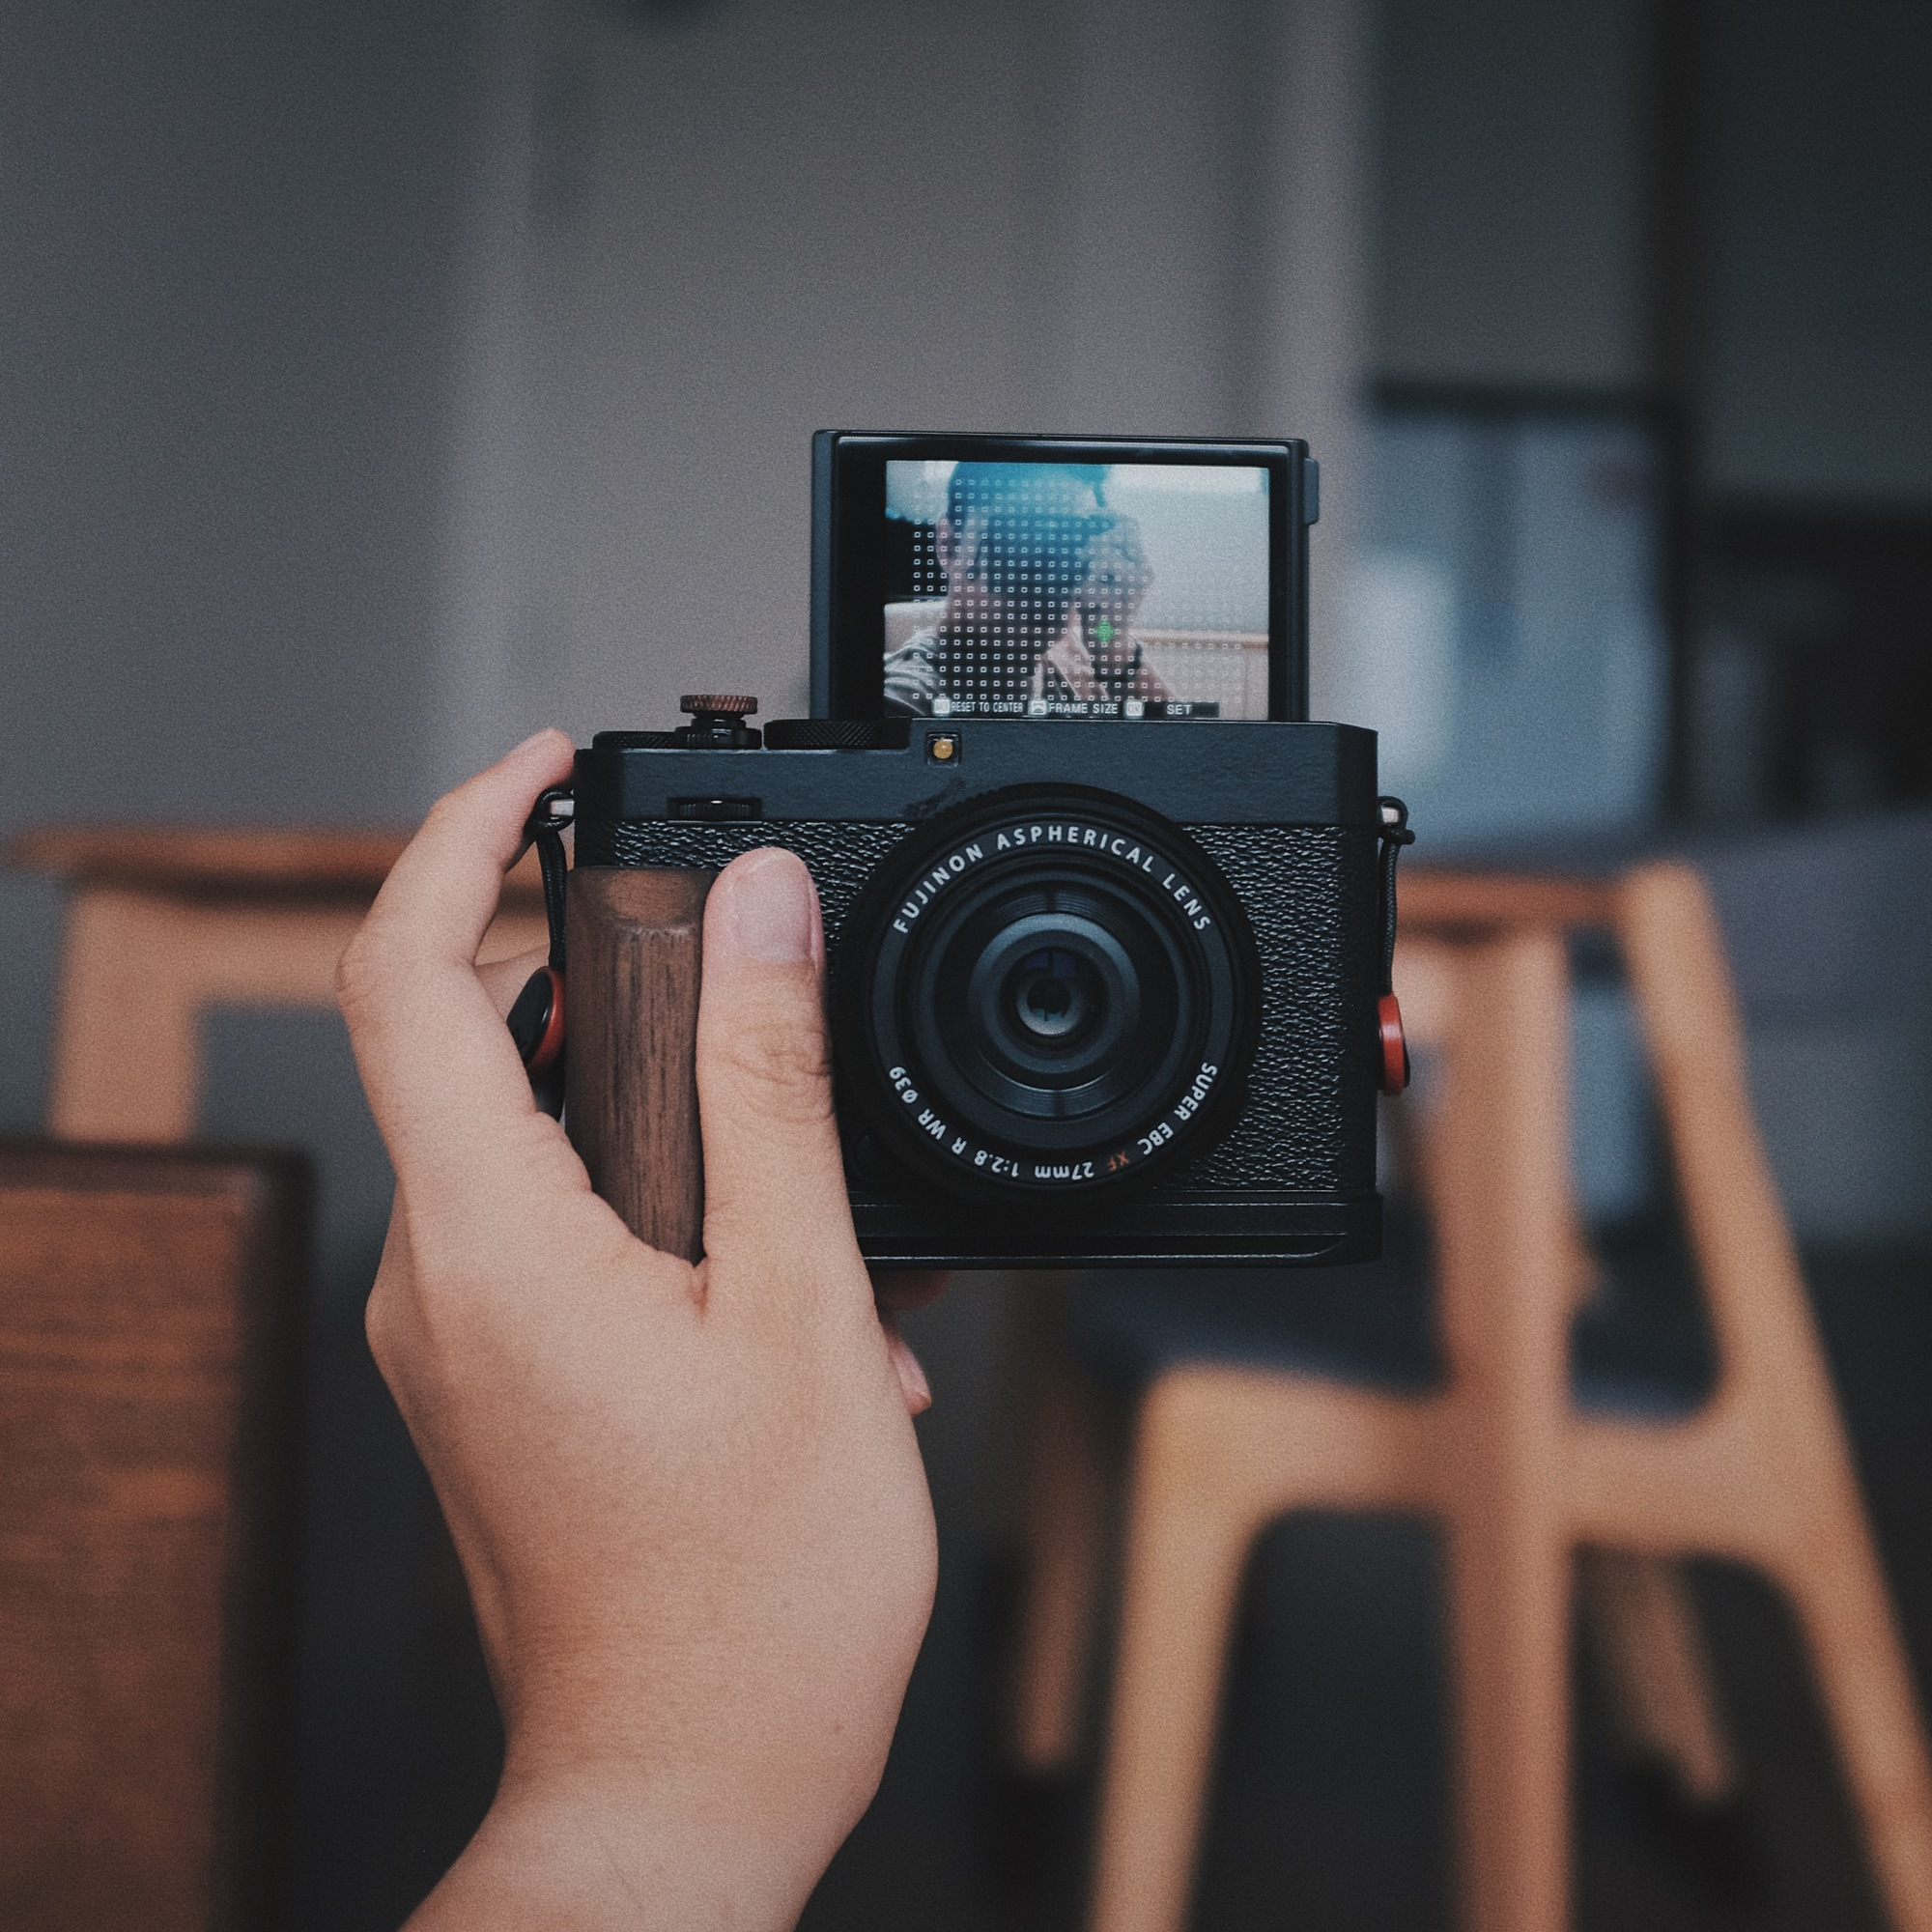
\includegraphics[width=\linewidth]{\envfinaldir/coverpic-prod.jpg}\par
            % \vskip 30pt
            \vfill

            \normalsize\rmfamily\scshape
            \copyright{} The Web Digest Project \hfill\large \envdatestr
        \end{center}
    \end{titlepage}
    % \restoregeometry
}
\newcommand{\simplehref}[1]{%
    \textcolor{blue!80!green}{\href{#1}{#1}}%
}
\renewcommand{\contentsname}{\center\Huge\sffamily\bfseries Contents\par\vskip 20pt}
\newcounter{ipartcounter}
\setcounter{ipartcounter}{0}
\newcommand{\ipart}[1]{
    % \vskip 20pt
    \clearpage
    \stepcounter{ipartcounter}
    \phantomsection
    \addcontentsline{toc}{chapter}{#1}
    % \begin{center}
    %     \Huge
    %     \sffamily\bfseries
    %     #1
    % \end{center}
    % \vskip 20pt plus 7pt
}
\newcounter{ichaptercounter}
\setcounter{ichaptercounter}{0}
\newcommand{\ichapter}[1]{
    % \vskip 20pt
    \clearpage
    \stepcounter{ichaptercounter}
    \phantomsection
    \addcontentsline{toc}{section}{\numberline{\arabic{ichaptercounter}}#1}
    \begin{center}
        \Huge
        \sffamily\bfseries
        #1
    \end{center}
    \vskip 20pt plus 7pt
}
\newcommand{\entrytitlefont}[1]{\subsection*{\raggedright\Large\sffamily\bfseries#1}}
\newcommand{\entryitemGeneric}[2]{
    % argv: title, url
    \parbox{\linewidth}{
        \entrytitlefont{#1}\par\vskip 5pt
        \footnotesize\ttfamily\mdseries
        \simplehref{#2}
    }\vskip 11pt plus 11pt minus 1pt
}
\newcommand{\entryitemGithub}[3]{
    % argv: title, url, desc
    \parbox{\linewidth}{
        \entrytitlefont{#1}\par\vskip 5pt
        \footnotesize\ttfamily\mdseries
        \simplehref{#2}\par\vskip 5pt
        \small\rmfamily\mdseries#3
    }\vskip 11pt plus 11pt minus 1pt
}
\newcommand{\entryitemAp}[3]{
    % argv: title, url, desc
    \parbox{\linewidth}{
        \entrytitlefont{#1}\par\vskip 5pt
        \footnotesize\ttfamily\mdseries
        \simplehref{#2}\par\vskip 5pt
        \small\rmfamily\mdseries#3
    }\vskip 11pt plus 11pt minus 1pt
}
\newcommand{\entryitemHackernews}[3]{
    % argv: title, hnurl, rawurl
    % \parbox{\linewidth}{
    %     \entrytitlefont{#1}\par\vskip 5pt
    %     \footnotesize\ttfamily\mdseries
    %     \simplehref{#3}\par
    %     \textcolor{black!50}{\href{#2}{#2}}
    % }\vskip 11pt plus 11pt minus 1pt
    \begin{minipage}{\linewidth}
            \entrytitlefont{#1}\par\vskip 5pt
            \footnotesize\ttfamily\mdseries
            \simplehref{#3}\par
            \textcolor{black!50}{\href{#2}{#2}}
    \end{minipage}\par\vskip 11pt plus 11pt minus 1pt
}







\begin{document}

\makeheader

\tableofcontents\clearpage




\ipart{Developers}
\ichapter{Hacker News}
\entryitemTwoLinks{Meta's live staged demo fails; the "AI" recording plays before the actor acts}{https://news.ycombinator.com/item?id=45294859}{https://old.reddit.com/r/LivestreamFail/comments/1nkbig7/metas\_live\_staged\_demo\_fails\_the\_ai\_recording/}

\entryitemTwoLinks{Apple: SSH and FileVault}{https://news.ycombinator.com/item?id=45294440}{https://keith.github.io/xcode-man-pages/apple\_ssh\_and\_filevault.7.html}

\entryitemTwoLinks{When Knowing Someone at Meta Is the Only Way to Break Out of "Content Jail"}{https://news.ycombinator.com/item?id=45293273}{https://www.eff.org/pages/when-knowing-someone-meta-only-way-break-out-content-jail}

\entryitemTwoLinks{This map is not upside down}{https://news.ycombinator.com/item?id=45292694}{https://www.maps.com/this-map-is-not-upside-down/}

\entryitemTwoLinks{Learn Your Way: Reimagining Textbooks with Generative AI}{https://news.ycombinator.com/item?id=45292648}{https://research.google/blog/learn-your-way-reimagining-textbooks-with-generative-ai/}

\entryitemTwoLinks{Chrome's New AI Features}{https://news.ycombinator.com/item?id=45292260}{https://blog.google/products/chrome/new-ai-features-for-chrome/}

\entryitemTwoLinks{Yes, Jimmy Kimmel's suspension was government censorship}{https://news.ycombinator.com/item?id=45292130}{https://www.theverge.com/policy/781148/jimmy-kimmel-charlie-kirk-monologue-brendan-carr-censorship-first-amendment}

\entryitemTwoLinks{Configuration files are user interfaces}{https://news.ycombinator.com/item?id=45291858}{https://ochagavia.nl/blog/configuration-files-are-user-interfaces/}

\entryitemTwoLinks{American Prairie unlocks another 70k acres in Montana}{https://news.ycombinator.com/item?id=45291132}{https://earthhope.substack.com/p/victory-for-public-access-american}

\entryitemTwoLinks{TernFS – An exabyte scale, multi-region distributed filesystem}{https://news.ycombinator.com/item?id=45290245}{https://www.xtxmarkets.com/tech/2025-ternfs/}

\entryitemTwoLinks{Grief gets an expiration date, just like us}{https://news.ycombinator.com/item?id=45290021}{https://bessstillman.substack.com/p/oh-fuck-youre-still-sad}

\entryitemTwoLinks{Geizhals Preisvergleich Donates USD 10k to the Perl and Raku Foundation}{https://news.ycombinator.com/item?id=45289834}{https://www.perl.com/article/geizhals-donates-to-tprf/}

\entryitemTwoLinks{Luau – Fast, small, safe, gradually typed scripting language derived from Lua}{https://news.ycombinator.com/item?id=45289558}{https://luau.org/}

\entryitemTwoLinks{Flipper Zero Geiger Counter}{https://news.ycombinator.com/item?id=45289453}{https://kasiin.top/blog/2025-08-04-flipper\_zero\_geiger\_counter\_module/}

\entryitemTwoLinks{The quality of AI-assisted software depends on unit of work management}{https://news.ycombinator.com/item?id=45289168}{https://blog.nilenso.com/blog/2025/09/15/ai-unit-of-work/}

\entryitemTwoLinks{KDE is now my favorite desktop}{https://news.ycombinator.com/item?id=45288690}{https://kokada.dev/blog/kde-is-now-my-favorite-desktop/}

\entryitemTwoLinks{You Had No Taste Before AI}{https://news.ycombinator.com/item?id=45288551}{https://matthewsanabria.dev/posts/you-had-no-taste-before-ai/}

\entryitemTwoLinks{Nvidia buys \$5B in Intel}{https://news.ycombinator.com/item?id=45288161}{https://www.tomshardware.com/pc-components/cpus/nvidia-and-intel-announce-jointly-developed-intel-x86-rtx-socs-for-pcs-with-nvidia-graphics-also-custom-nvidia-data-center-x86-processors-nvidia-buys-usd5-billion-in-intel-stock-in-seismic-deal}

\entryitemTwoLinks{This website has no class}{https://news.ycombinator.com/item?id=45287155}{https://aaadaaam.com/notes/no-class/}

\entryitemTwoLinks{Pnpm has a new setting to stave off supply chain attacks}{https://news.ycombinator.com/item?id=45286526}{https://pnpm.io/blog/releases/10.16}\ichapter{Phoronix}
\entryitemGeneric{\hskip 0pt{}Revisiting DDR5-6400 vs. MRDIMM-8800 Performance With Intel Xeon 6 "Granite Rapids"}{https://www.phoronix.com/review/ddr5-6400-mrdimm-8800}

\entryitemGeneric{\hskip 0pt{}Rust 1.90 Released With LLD Default On Linux x86\_64 While macOS x86\_64 Demoted}{https://www.phoronix.com/news/Rust-1.90-Released}

\entryitemGeneric{\hskip 0pt{}Python 3.14-rc3 Released Ahead Of Next Month's Official Release}{https://www.phoronix.com/news/Python-3.14-rc3-Released}

\entryitemGeneric{\hskip 0pt{}NVIDIA To Make \$5B Investment Into Intel - x86 RTX SoCs \& More To Come}{https://www.phoronix.com/news/NVIDIA-Intel-5B-Investment}

\entryitemGeneric{\hskip 0pt{}Linux Mint Releases LMDE 7 Beta}{https://www.phoronix.com/news/Linux-Mint-LMDE-7-Beta}

\entryitemGeneric{\hskip 0pt{}Fedora Forge Announced For Modernizing Fedora's Development \& Collaboration}{https://www.phoronix.com/news/Fedora-Forge}

\entryitemGeneric{\hskip 0pt{}Linux 6.17 AMD PMF Driver Adding New ACPI ID For Upcoming AMD Platform}{https://www.phoronix.com/news/Linux-6.17-AMD-AMDI0108}

\entryitemGeneric{\hskip 0pt{}Microchip LAN969x SoC Going Upstream In Linux 6.18}{https://www.phoronix.com/news/Microchip-LAN969x-Linux-6.18}

\entryitemGeneric{\hskip 0pt{}Intel's Latest Open-Source Project To End \& Layoff Developers... But A New Home At NumPy}{https://www.phoronix.com/news/Intel-NumPy-x86-simd-sort}


\ipart{Developers~~~~(zh-Hans)}
\ichapter{Solidot}
\entryitemGeneric{\hskip 0pt{}研究发现珊瑚无法在一个更温暖的世界里生存下来}{https://www.solidot.org/story?sid=82355}

\entryitemGeneric{\hskip 0pt{}DeepSeek 发表 R1 模型论文,称训练成本仅 29.4 万美元}{https://www.solidot.org/story?sid=82354}

\entryitemGeneric{\hskip 0pt{}全球变暖致日本危险性高温日增加 22 天}{https://www.solidot.org/story?sid=82353}

\entryitemGeneric{\hskip 0pt{}NASA 确认了逾六千颗系外行星}{https://www.solidot.org/story?sid=82352}

\entryitemGeneric{\hskip 0pt{}最黑暗的夜晚愈来愈亮}{https://www.solidot.org/story?sid=82351}

\entryitemGeneric{\hskip 0pt{}电视的黄金时代可能已经结束}{https://www.solidot.org/story?sid=82350}

\entryitemGeneric{\hskip 0pt{}极端高温催生新法律保护工人}{https://www.solidot.org/story?sid=82349}

\entryitemGeneric{\hskip 0pt{}美国国会要求 Valve、Discord 和 Twitch CEO 就用户激进化作证}{https://www.solidot.org/story?sid=82348}

\entryitemGeneric{\hskip 0pt{}小鹏汇天两辆飞行汽车在长春航展上相撞}{https://www.solidot.org/story?sid=82347}

\entryitemGeneric{\hskip 0pt{}GNOME 49 释出}{https://www.solidot.org/story?sid=82346}

\entryitemGeneric{\hskip 0pt{}黑猩猩每天食用熟果摄入的酒精量相当于一瓶啤酒}{https://www.solidot.org/story?sid=82345}

\entryitemGeneric{\hskip 0pt{}ChatGPT 将估计用户年龄,可能要求验证年龄}{https://www.solidot.org/story?sid=82344}

\entryitemGeneric{\hskip 0pt{}迪士尼华纳等起诉中国 AI 公司侵犯版权}{https://www.solidot.org/story?sid=82343}

\entryitemGeneric{\hskip 0pt{}气候暖化会让土壤释放出更多碳}{https://www.solidot.org/story?sid=82342}

\entryitemGeneric{\hskip 0pt{}字节跳动阿里巴巴等公司被要求停止购买英伟达 AI 芯片}{https://www.solidot.org/story?sid=82341}

\entryitemGeneric{\hskip 0pt{}NPM 再次发现供应链攻击 }{https://www.solidot.org/story?sid=82340}

\entryitemGeneric{\hskip 0pt{}M87*黑洞图像显示其偏振方向发生翻转}{https://www.solidot.org/story?sid=82339}

\entryitemGeneric{\hskip 0pt{}Firefox 143.0 释出}{https://www.solidot.org/story?sid=82338}

\entryitemGeneric{\hskip 0pt{}白垩纪兽脚类恐龙奔跑时速能达到 45 公里}{https://www.solidot.org/story?sid=82337}

\entryitemGeneric{\hskip 0pt{}AMD 终止自己的 AMDVLK 开源驱动项目,拥抱社区项目 Mesa RADV}{https://www.solidot.org/story?sid=82336}\ichapter{V2EX}
\entryitemGeneric{\hskip 0pt{}[经济] 房地产泡沫如何形成?}{https://www.v2ex.com/t/1160364}

\entryitemGeneric{\hskip 0pt{}[Apple] 如果乔布斯活到今天}{https://www.v2ex.com/t/1160363}

\entryitemGeneric{\hskip 0pt{}[分享发现] 36 岁开始,每日提肛 500 下,这个数管住了我,不会胡思乱想}{https://www.v2ex.com/t/1160362}

\entryitemGeneric{\hskip 0pt{}[Apple] 有什么办法可以将 apple.com.cn 的 cdn 解析到国内 IP 呢}{https://www.v2ex.com/t/1160361}

\entryitemGeneric{\hskip 0pt{}[职场话题] 大公司会要求入职体检吗?}{https://www.v2ex.com/t/1160360}

\entryitemGeneric{\hskip 0pt{}[Android] 红米 k50 从 HyperOS 2 降回 MIUI 14 后}{https://www.v2ex.com/t/1160358}

\entryitemGeneric{\hskip 0pt{}[分享发现] 这可能是我最近几年买的最好玩的电子垃圾了,爱普生 L1455 全功能打印机}{https://www.v2ex.com/t/1160357}

\entryitemGeneric{\hskip 0pt{}[程序员] [trae] 不想续费了}{https://www.v2ex.com/t/1160356}

\entryitemGeneric{\hskip 0pt{}[Cursor] Claude Code 已经替代 Cursor 使用两个月了,但是还离不开它的自动补全, VSCode 的自动补全赶上来了吗?}{https://www.v2ex.com/t/1160354}

\entryitemGeneric{\hskip 0pt{}[分享创造] 在线文件夹/文件比较工具, Beyond Compare alternative}{https://www.v2ex.com/t/1160353}

\entryitemGeneric{\hskip 0pt{}[宽带症候群] 联通 168 小时固定重启,有什么办法吗?}{https://www.v2ex.com/t/1160352}

\entryitemGeneric{\hskip 0pt{}[浏览器] 浏览器迁移好麻烦}{https://www.v2ex.com/t/1160351}

\entryitemGeneric{\hskip 0pt{}[问与答] 现在 docker hub 国内可用的镜像有推荐吗?}{https://www.v2ex.com/t/1160350}

\entryitemGeneric{\hskip 0pt{}[程序员] 只有一台笔记本电脑,真的可以长时间编程吗?(无外接显示器)}{https://www.v2ex.com/t/1160349}

\entryitemGeneric{\hskip 0pt{}[分享创造] 做了个版权符号的网站}{https://www.v2ex.com/t/1160348}

\entryitemGeneric{\hskip 0pt{}[酷工作] 项目名称: H5 + PWA 播放器 Demo 开发(JSON + VTT 渲染验证版)}{https://www.v2ex.com/t/1160346}

\entryitemGeneric{\hskip 0pt{}[杭州] 有人需要租大江东的房子吗? 139 平四居室包车位,房东直租}{https://www.v2ex.com/t/1160342}

\entryitemGeneric{\hskip 0pt{}[Solana] 请问 签到的 金币 银币 可以转为\$v2ex 币吗?}{https://www.v2ex.com/t/1160341}

\entryitemGeneric{\hskip 0pt{}[阅读] 我也找一篇文章,应该是微型小说}{https://www.v2ex.com/t/1160340}

\entryitemGeneric{\hskip 0pt{}[健身] 户晨风说 减肥就是要靠挨饿,节食}{https://www.v2ex.com/t/1160338}

\entryitemGeneric{\hskip 0pt{}[问与答] wps 国际版是不是不能用 wps 国内版的超级会员?}{https://www.v2ex.com/t/1160337}

\entryitemGeneric{\hskip 0pt{}[分享发现] 各种样式风格的图片、视频生成的太多了,所以做了一个汇总的图片视频生成网站}{https://www.v2ex.com/t/1160336}

\entryitemGeneric{\hskip 0pt{}[NAS] 5 月从某鱼买的硬盘,坏了俩}{https://www.v2ex.com/t/1160335}

\entryitemGeneric{\hskip 0pt{}[CDN] 请问下 CDN 推荐哪家}{https://www.v2ex.com/t/1160334}

\entryitemGeneric{\hskip 0pt{}[分享创造] 做了一个生成随机数的网站}{https://www.v2ex.com/t/1160333}

\entryitemGeneric{\hskip 0pt{}[问与答] 其实我纯吐槽的,笔记本风扇好吵}{https://www.v2ex.com/t/1160331}

\entryitemGeneric{\hskip 0pt{}[职场话题] 从沪漂到郑漂:我用``最小成本创业'',还清房贷、拥抱家庭}{https://www.v2ex.com/t/1160329}

\entryitemGeneric{\hskip 0pt{}[分享发现] Neon 免费数据库时间翻倍了?}{https://www.v2ex.com/t/1160328}

\entryitemGeneric{\hskip 0pt{}[PHP] 求助: PHP 错误,请高手帮我改写下面的 PHP 代码}{https://www.v2ex.com/t/1160327}

\entryitemGeneric{\hskip 0pt{}[分享发现] 使用广电手机卡流量在 12306 上无法抢票,提示您的设备环境异常。}{https://www.v2ex.com/t/1160325}

\entryitemGeneric{\hskip 0pt{}[Docker] 请教一个 Docker/Traefik 的网路问题}{https://www.v2ex.com/t/1160324}

\entryitemGeneric{\hskip 0pt{}[VPS] 收 DMIT.HKG.Pro}{https://www.v2ex.com/t/1160323}

\entryitemGeneric{\hskip 0pt{}[问与答] 不要运营商信号,只使用 Wi-Fi Calling 的电话卡有什么选择}{https://www.v2ex.com/t/1160322}

\entryitemGeneric{\hskip 0pt{}[宽带症候群] 求推荐一个丢国外免维护超高可靠的软路由软/硬方案}{https://www.v2ex.com/t/1160321}

\entryitemGeneric{\hskip 0pt{}[问与答] 问下现在国内的空调什么空调温控好呢?}{https://www.v2ex.com/t/1160320}

\entryitemGeneric{\hskip 0pt{}[问与答] 现在在 app store 买 Claude Pro 稳定吗}{https://www.v2ex.com/t/1160319}

\entryitemGeneric{\hskip 0pt{}[问与答] iPhone 17 和 pro 之间的价格差距足够买一个相机来弥补吗? 纯比较影像的话}{https://www.v2ex.com/t/1160318}

\entryitemGeneric{\hskip 0pt{}[推广] 腾讯云轻量续费拼团}{https://www.v2ex.com/t/1160316}

\entryitemGeneric{\hskip 0pt{}[健康] 你们小时候有被家长带去扎手指吗?}{https://www.v2ex.com/t/1160314}

\entryitemGeneric{\hskip 0pt{}[问与答] 移动脉率房颤和房颤历史开哪个?}{https://www.v2ex.com/t/1160313}

\entryitemGeneric{\hskip 0pt{}[分享发现] 玩了几天刷 esim,挺好玩}{https://www.v2ex.com/t/1160312}

\entryitemGeneric{\hskip 0pt{}[Apple] 把 Launchpad 带回 macOS 26 的又一款程序}{https://www.v2ex.com/t/1160311}

\entryitemGeneric{\hskip 0pt{}[生活] [记录]-2025-09-17 第二次骑车挂彩}{https://www.v2ex.com/t/1160309}

\entryitemGeneric{\hskip 0pt{}[生活] 六天爬完黄山五岳,我可以给出以下信息}{https://www.v2ex.com/t/1160308}

\entryitemGeneric{\hskip 0pt{}[海口] LOVEMONEY}{https://www.v2ex.com/t/1160307}

\entryitemGeneric{\hskip 0pt{}[分享创造] LoveMoney Game}{https://www.v2ex.com/t/1160305}

\entryitemGeneric{\hskip 0pt{}[Chrome] night eye 这个插件真好用,有没有便宜的订阅渠道}{https://www.v2ex.com/t/1160304}

\entryitemGeneric{\hskip 0pt{}[Solana] 站内打赏的 24 小时的大致流量}{https://www.v2ex.com/t/1160303}

\entryitemGeneric{\hskip 0pt{}[iPhone] 更新了 iOS26 发现需要 FQ 的网站打开特别慢,要等一会儿才能完全打开}{https://www.v2ex.com/t/1160302}

\entryitemGeneric{\hskip 0pt{}[问与答] 币安每次登陆都要人脸,包括转账也是}{https://www.v2ex.com/t/1160301}


\ipart{Generic News}







\clearpage
\leavevmode\vfill
\footnotesize

Copyright \copyright{} 2023-2025 Neruthes and other contributors.

This document is published with CC BY-NC-ND 4.0 license.

The entries listed in this newsletter may be copyrighted by their respective creators.

This newsletter is generated by the Web Digest project.

The newsletters are also delivered via Telegram channel \CJKunderline{\href{https://t.me/webdigestchannel}{https://t.me/webdigestchannel}}.\\
RSS feed is available at \CJKunderline{\href{https://webdigest.pages.dev/rss.xml}{https://webdigest.pages.dev/rss.xml}}.

This newsletter is available in PDF at
\CJKunderline{\href{https://webdigest.pages.dev/}{https://webdigest.pages.dev/}}.

The source code being used to generate this newsletter is available at\\
\CJKunderline{\href{https://github.com/neruthes/webdigest}{https://github.com/neruthes/webdigest}}.

This newsletter is also available in
\CJKunderline{\href{http://webdigest.pages.dev/readhtml/\envyear/WebDigest-20250919.html}{HTML}} and
\CJKunderline{\href{https://github.com/neruthes/webdigest/blob/master/markdown/\envyear/WebDigest-20250919.md}{Markdown}}.


\coverpic{https://unsplash.com/photos/large-green-leaves-of-a-plant-against-a-tan-wall-Znn0VgKgo4c}{Fujiphilm}


\end{document}
